\documentclass[]{article}
\usepackage{lmodern}
\usepackage{amssymb,amsmath}
\usepackage{ifxetex,ifluatex}
\usepackage{fixltx2e} % provides \textsubscript
\ifnum 0\ifxetex 1\fi\ifluatex 1\fi=0 % if pdftex
  \usepackage[T1]{fontenc}
  \usepackage[utf8]{inputenc}
\else % if luatex or xelatex
  \ifxetex
    \usepackage{mathspec}
  \else
    \usepackage{fontspec}
  \fi
  \defaultfontfeatures{Ligatures=TeX,Scale=MatchLowercase}
\fi
% use upquote if available, for straight quotes in verbatim environments
\IfFileExists{upquote.sty}{\usepackage{upquote}}{}
% use microtype if available
\IfFileExists{microtype.sty}{%
\usepackage{microtype}
\UseMicrotypeSet[protrusion]{basicmath} % disable protrusion for tt fonts
}{}
\usepackage[margin=1in]{geometry}
\usepackage{hyperref}
\hypersetup{unicode=true,
            pdftitle={A national, multi-decadal, water quality and Landsat dataset},
            pdfauthor={Matthew Ross and lots of others!},
            pdfborder={0 0 0},
            breaklinks=true}
\urlstyle{same}  % don't use monospace font for urls
\usepackage{graphicx,grffile}
\makeatletter
\def\maxwidth{\ifdim\Gin@nat@width>\linewidth\linewidth\else\Gin@nat@width\fi}
\def\maxheight{\ifdim\Gin@nat@height>\textheight\textheight\else\Gin@nat@height\fi}
\makeatother
% Scale images if necessary, so that they will not overflow the page
% margins by default, and it is still possible to overwrite the defaults
% using explicit options in \includegraphics[width, height, ...]{}
\setkeys{Gin}{width=\maxwidth,height=\maxheight,keepaspectratio}
\IfFileExists{parskip.sty}{%
\usepackage{parskip}
}{% else
\setlength{\parindent}{0pt}
\setlength{\parskip}{6pt plus 2pt minus 1pt}
}
\setlength{\emergencystretch}{3em}  % prevent overfull lines
\providecommand{\tightlist}{%
  \setlength{\itemsep}{0pt}\setlength{\parskip}{0pt}}
\setcounter{secnumdepth}{0}
% Redefines (sub)paragraphs to behave more like sections
\ifx\paragraph\undefined\else
\let\oldparagraph\paragraph
\renewcommand{\paragraph}[1]{\oldparagraph{#1}\mbox{}}
\fi
\ifx\subparagraph\undefined\else
\let\oldsubparagraph\subparagraph
\renewcommand{\subparagraph}[1]{\oldsubparagraph{#1}\mbox{}}
\fi

%%% Use protect on footnotes to avoid problems with footnotes in titles
\let\rmarkdownfootnote\footnote%
\def\footnote{\protect\rmarkdownfootnote}

%%% Change title format to be more compact
\usepackage{titling}

% Create subtitle command for use in maketitle
\newcommand{\subtitle}[1]{
  \posttitle{
    \begin{center}\large#1\end{center}
    }
}

\setlength{\droptitle}{-2em}

  \title{A national, multi-decadal, water quality and Landsat dataset}
    \pretitle{\vspace{\droptitle}\centering\huge}
  \posttitle{\par}
    \author{Matthew Ross and lots of others!}
    \preauthor{\centering\large\emph}
  \postauthor{\par}
      \predate{\centering\large\emph}
  \postdate{\par}
    \date{October 22, 2018}

\usepackage{booktabs}
\usepackage{longtable}
\usepackage{array}
\usepackage{multirow}
\usepackage[table]{xcolor}
\usepackage{wrapfig}
\usepackage{float}
\usepackage{colortbl}
\usepackage{pdflscape}
\usepackage{tabu}
\usepackage{threeparttable}
\usepackage{threeparttablex}
\usepackage[normalem]{ulem}
\usepackage{makecell}

\begin{document}
\maketitle

{
\setcounter{tocdepth}{2}
\tableofcontents
}
\hypertarget{introduction}{%
\section{Introduction}\label{introduction}}

The production of and easy access to water quality data is a vital first
step towards understanding natural and anthropogenic drivers of aquatic
ecosystem degradation and for using this knowledge to protect and manage
inland waters (Srebotnjak et al., 2012). Collecting such valuable data
has historically been expensive and time-consuming, and it has often
proved difficult to maintain useable and open datasets. In many
developed nations, however, over the last 10-20 years many of these data
access problems have been actively addressed, leading to the publication
and maintenance of large open-access data repositories of water quality
measurements (Ballantine \& Davies-Colley, 2014; Lack, 2000; Read et
al., 2017; Soranno et al., 2017). Although they contain millions of
individual measurements, these datasets remain limited to the relatively
time-intensive process of field sampling, which limits the number of
water-bodies that can be observed and the spatial variation in water
quality captured within a single waterbody. Furthermore, access to such
robust historic water quality sampling data remains limited to a few
economically developed countries. With satellite remote sensing
detection of water quality, we can augment these \emph{in-situ} sampling
efforts and provide water quality information in places with little or
no data.

Since the beginning of the Landsat missions, limnologists,
oceanographers, and hydrologists have been interested in developing
universal algorithms for extracting water quality information from
remotely sensed images (Clarke et al., 1970; Holyer, 1978; Klemas et
al., 1973; Maul \& Gordon, 1975; Ritchie et al., 1976). Since these
early efforts, there has been almost fifty years of work with the basic
goal of using spectral information to predict water quality parameters
like total suspended solids (TSS), Chlorophyll a (Chl\_a), colored
dissolved organic matter (CDOM), and Secchi disk depth (SDD). However,
progress towards universal algorithms and unified approaches has been
slow (Blondeau-Patissier et al., 2014; Bukata, 2013; Gholizadeh et al.,
2016), with most papers published focusing on developing predictive
methods as opposed to using predictions to interrogate processes that
control water quality dynamics (Topp et al., 2018). Furthermore, most of
the datasets used in these prior studies are inherently local in scale,
often sampling a single waterbody on a single day corresponding to a
satellite overpass (Topp et al., 2018). These limited datasets have
contributed to the slow evolution in methods and approaches along with
the inherent optical complexity of inland waters, where spectral
signatures reflect a mixture of inorganic sediment, organic sediment,
algae, dissolved organic matter, and other constituents. Compared to
oceanic remote sensing of water quality which benefits from robust, open
datasets paired with satellite overpass reflectance (Blondeau-Patissier
et al., 2014; Bukata, 2013), progress on inland water algorithms is
impeded by this lack of an open, merged satellite reflectance and
\emph{in-situ} water quality dataset. Such a dataset would facilitate
more unified approaches to water quality remote sensing, ideally
simplifying algorithm development to the point where remote estimates of
water quality are integrated into our approaches for understanding
inland water quality dynamics and their controls.

Here, we create and share a merged dataset, AquaSat, of water quality
measurements and same-day satellite reflectance (which we call
``overpasses''). This is the largest such overpass dataset ever
assembled for inland waters. We use the Landsat TM/ETM+/OLI archive from
1984-2018 using the using the Google Earth Engine platform (Gorelick et
al., 2017) in combination with data from the Water Quality Portal (Read
et al., 2017) and phase one of the \emph{LAke multi-scaled GeOSpatial
and temporal database}, with data only in the Northeastern United States
(LAGOS-NE)(Soranno et al., 2017). The WQP data covers the conterminous
USA and Alaska. Joining these datasets provides us with an unprecedented
resource to model, predict, and understand the long-term and large-scale
dynamics of variation in four key water clarity constituents: TSS, SDD,
Chl\_a, and dissolved organic carbon (DOC). We also outline and share
our approach, code, and intermediate data for bringing these three free
datasets together; generating a high-graded analysis-ready dataset for
remote sensors of water quality. We hope that publishing the code will
encourage developing similar matchup datasets for public water quality
datasets like in New Zealand (Ballantine \& Davies-Colley, 2014) or
Europe(Lack, 2000).

\hypertarget{methods}{%
\section{Methods}\label{methods}}

\hypertarget{parameter-description}{%
\subsection{Parameter description}\label{parameter-description}}

For this project we chose to focus on the four most common water quality
parameters used in remote sensing of water quality: TSS, SDD, Chl\_a,
and DOC {[}Topp et al., 2018{]}. All four of these parameters provide
useful and complimentary information on the water quality status of a
waterbody and are also optically active, making them observable from
space. TSS is a measure of the mass of solids, both organic and
inorganic, in a water column. Waters with higher TSS generally scatter
more sunlight at all visible and near-infrared wavelengths (Ritchie et
al., 1976). Knowing TSS concentrations can provide insight into light
conditions (Julian et al., 2008), erosion conditions {[}Syvitski2011{]},
and the hydrologic status of waterbodies, where high TSS generally means
high flow velocities {[}Williams (1989);Pavelsky2009{]}. DOC is the
broad description for the total amount of organic Carbon that is
dissolved in water, and can provide insight into light conditions
(Vähätalo et al., 2005), heterotrophic energy availability (Robbins et
al., 2017), and terrestrial organic matter processing (Williamson et
al., 2008). While DOC does not inherently alter the optical properties
of water, it is generally strongly correlated with CDOM, which is
optically active, generally a brown or yellow color (Bricaud et al.,
1981; Griffin et al., 2011). Though this correlation between CDOM and
DOC can breakdown in places with low DOC concentratnio (Griffin et al.,
2018). For this project, we included both DOC and CDOM data. Chlorophyll
a is a photosynthetically active pigment contained in all phytoplankton,
which helps give algal blooms their green color. Chlorophyll a
concentrations can be used to detect algae blooms (Kutser, 2004),
estimate primary productivity (Antoine et al., 1996), and understand
algae dynamics (Richardson, 1996). Finally, we gathered data on Secchi
disk depth, a long-standing method for estimating water clarity (Secchi,
1864). The Secchi disk is a 30 cm diameter disk divided into four
quadrants painted alternately white and black. To measure water clarity,
the disk is lowered into a waterbody; the depth at which the disk is no
longer visible is the Secchi disk depth. Deeper depths mean clearer
water. Secchi disk depth is a simple measurement that integrates the
optical properties of all water constituents and can provide information
on the trophic status of waterbodies (Carlson, 1977) or the algae status
of a waterbody (Lorenzen, 1980). These four parameters capture key
ecological and physical factors that control water quality, and
capabilities to remotely sense each of them have been demonstrated in
many studies (Topp et al., 2018), making them ideal for our dataset
construction efforts.

\hypertarget{data-source-description}{%
\subsection{Data source description}\label{data-source-description}}

Combining \emph{in-situ} data with Landsat reflectance information first
requires a large repository of water quality samples, which increases
the likelihood that a given sample happened to be taken on the same day
as a Landsat overpass. For this paper, we focused on the two largest
databases of water quality in the United States. The first, the Water
Quality Portal has tens of millions of water observations in all types
of inland surface waters. The WQP data is gathered by a range of
national and state agencies (USGS, EPA, state water quality programs).
While there is no entity that harmonizes and cleans the data across
systems and data providers (Read et al., 2017), subsets of the data have
been used in many previous publications (Booth et al., 2011; Sprague \&
Lorenz, 2009; Sprague et al., 2017). The second dataset, LAGOS-NE,
currently only covers lakes in the northeastern United States (Soranno
et al., 2017). While LAGOS-NE has less data than the WQP, with more than
a million total observations, a group of dedicated researchers has spent
years ensuring data quality, making it a more analysis-ready dataset
(Soranno et al., 2017). These similar but contrasting datasets, one with
more quantity (WQP) and the other with more quality assurances
(LAGOS-NE), ensures that our dataset covers the largest possible number
of waterbodies, while retaining a high quality subset of the data.

\hypertarget{water-quality-portal}{%
\subsubsection{Water Quality Portal}\label{water-quality-portal}}

The WQP is the largest dataset of water observations ever assembled with
more than 290 million observations at 2.7 million sites dating back more
than a century, mostly in the USA (Read et al., 2017). The WQP
continuously gathers water quality information from more than 450
organizations including academic, government, NGO, tribal, and state
datasets (Read et al., 2017). These datastreams are gathered and
distributed in a standardized format, making analysis across different
collection methods more readily available. As with many large datasets,
however, the diversity of data sources and variation in meta-data
quality results in some significant challenges to directly using the WQP
as an analysis-ready dataset (Sprague et al., 2017). Instead, end-users
must carefully harmonize data across sampling methods, analytic
approaches, and units. The nature of harmonizing such large, distributed
data generates a necessary trade-off between a deep, time-consuming
exploration of data interoperability and a shallower less time-consuming
but potentially more error-prone data quality check.

\hypertarget{lagos-ne}{%
\subsubsection{LAGOS-NE}\label{lagos-ne}}

The LAGOS project (which generated the dataset LAGOS-NE) was, in part,
meant as a direct way to address some of the problems inherent to the
WQP, with the explicit goal of building a publically available
high-quality dataset for continental-scale lake analyses (Soranno et
al., 2017, 2015). In addition to pairing \emph{in-situ} lake data with
physical lake characteristics and local geologic setting, LAGOS
researchers standardized key water quality measurements across the 87
water quality datasets that they gathered (Soranno et al., 2017, 2015).
Because LAGOS researchers harmonized data from many different sources,
they chose to identify all data for a single lake with the lake
centroid. If two different organizations were measuring Secchi disk
depth at the north and south end of a lake, the LAGOS dataset would
combine all of these measurements into a single time series,
geographically located at the lake centroid, for same day observations
the deepest observation would have been kept (Soranno et al., 2015).
This approach is different from that used by the Water Quality Portal,
which often includes multiple sites per water body and simiultaneous
observations. In its current form, the LAGOS-NE dataset covers only
lakes in the northeast and midwest, two lake-rich regions of the USA.
LAGOS-NE provides an end-member dataset of the highest quality for
matching \emph{in-situ} data to Landsat overpasses.

\hypertarget{landsat}{%
\subsubsection{Landsat}\label{landsat}}

For this project, we join these two \emph{in-situ} datasets with the
Landsat data archive for Landsat missions 5 (Thematic Mapper), 7
(Enhanced Thematic Mapper +), and 8 (Operational Land Imager). . The
Landsat missions started in July 1972, as the Earth Resources
Observation Satellite with an explicit mission to provide solutions for
some of earth's pressing issues associated with industry and
environmental change (Loveland \& Dwyer, 2012). For this project we are
only using the three most recent Landsat mission datasets: Landsat 5
with coverage from 1984-2012 and over 192745 available images; Landsat 7
which is still collecting data after launching in July of 1999 with
191366 images; and finally Landsat 8 which launched in November, 2013
still adding to its collection of 61790 images. The total usable images
will be much less than the total images because of cloud cover, which
varies greatly by region. Furthermore, on May 31, 2003, the Landsat 7
scan line corrector failed, causing the Landsat 7 images after this date
to have striped data gaps (Storey et al., 2005). We included all Landsat
7 data before and after this date, but did not fill gaps associated with
the scan line error. The orbit repeat period of all three satellites is
sixteen days, though at high latitudes overlapping images result in
shorter revisit times (Loveland \& Dwyer, 2012; Wulder et al., 2016). In
most of the USA, a given spot will be imaged at least once every sixteen
days, and during periods of mission overlap, images are available on
average at least every eight days.

Landsat 5 and 7 have onboard imagers that collects seven bands of
imagery centered on three visible wavelengths (blue, green, and red) and
four infrared (near infrared, shortwave infrared 1, shortwave infrared
2, and thermal band). Landsat 8 has the same bands with slightly
different wavelengths and improved spectral accuracy (Barsi et al.,
2014) plus a few extra bands that we did not include in this work.
Landsat 7 and 8 have panchromatic bands at 15m resolution, while Landsat
5 does not. For our matchup data, the bands we used, their wavelengths,
and resolution are in SI table 1.

\hypertarget{data-integration}{%
\subsection{Data integration}\label{data-integration}}

The goal of uniting the WQP, LAGOS-NE and Landsat datasets requires a
combination of computational approaches and an architecture that allows
for a single workflow to download data from all three portals. An ideal
overarching approach allows us to break the various data downloads,
quality assurance checks, and joining data into separate pieces that can
be updated only as needed. In developing this approach, we emphasize not
only the possibilities that come with open data, but also the importance
of reproducible science and code. Here we chose to use a ``MAKE'' like
environment (Feldman, 1979) that only executes sections of code that
have been altered or when data sources are out of date. Though this
project uses three different tools (R, Python, and Google Earth Engine),
each tool is called directly from R and RMarkdown files. This reliance
on R makes remake \url{https://github.com/richfitz/remake} an excellent
choice to keep track of changes to the complex commands required to
compile AquaSat. Remake provides an R-specific, MAKE-like environment
that can check if code has been updated and then update all downstream
data. We anticipate that these efforts will make recreating or altering
our specific approach easier for future researchers who may want to use
our code in different ways. The detailed process of data integration is
captured in Figure \ref{fig:fig1}.

\begin{figure}
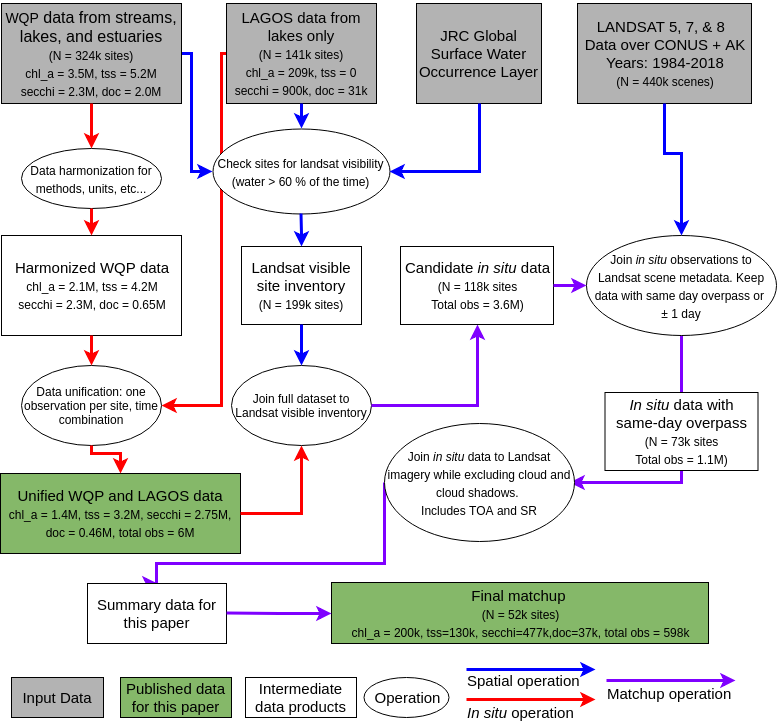
\includegraphics[width=0.8\linewidth]{C:/Users/mrvr/Dropbox/UNC-PostDocAll/aquasat/4_report/src/Watersat_Drop_flow} \caption{Overview of data sources, steps taken to join data, and total observation counts}\label{fig:fig1}
\end{figure}

\hypertarget{in-situ-data-download-and-quality-control.}{%
\subsubsection{\texorpdfstring{\emph{In situ} data download and quality
control.}{In situ data download and quality control.}}\label{in-situ-data-download-and-quality-control.}}

To begin the development of the AquaSat database, we developed an
automated method to retrieve our four water quality parameters from the
WQP and LAGOS sites. For the WQP we used the
\href{https://github.com/USGS-R/dataRetrieval}{dataRetrieval} R package.
DataRetrieval, maintained and supported by the USGS, which allows for
systematically downloading data from the WQP. The WQP contains hundreds
of parameter types (under the field ``characteristicName'' in the WQP),
and we carefully selected those that best represented our target
parameters based on our own expertise and previously published research
using the same data sources (Butman et al., 2016; Stets \& Striegl,
2012)(SI Table 2). For all parameters, we downloaded data for all US
states except Hawaii. The WQP classifies water body types in many
possible categories and we downloaded data for the four following water
body types: Lake, Reservoir, Impoundment; Stream; Estuary; Facility,
where facility can indicate wastewater treatment facilities, including
lakes and ponds. Finally, we restricted our queries to data sampled in
water as a sample media, excluding sediment and benthic samples.

Working with the LAGOS-NE data (version 1.087.1) required many less
decisions to combine parameters since LAGOS researchers have already
harmonized and combined parameters into simple categories that reflect
our general parameter codes(Soranno et al., 2017, 2015). LAGOS-NE
includes measurements of: DOC, Chl\_a, and SDD, but no data on TSS. As
with the WQP the dataset can be simply loaded using an R package
(`LAGOS-NE')(Soranno et al., 2017).

Turning data from the WQP into an analysis-ready dataset similar to
LAGOS-NE requires a chain of decisions that is extensively documented in
the supplemental \href{link}{website}. We have attempted to make these
decisions both clear and justifiable, with the end goal of producing a
high-quality dataset. Figure \ref{fig:fig1} presents these data quality
assurance procedures and shows how they reduce the number of
observatiosn at each step. The following are the most important
decisions:

\begin{enumerate}
\def\labelenumi{\arabic{enumi}.}
\item
  All observations were verified to have analytical methods that matched
  their parameter name; when this was not the case, samples were
  dropped. For example, if an observation was supposed to report TSS,
  but the analytical method was listed as ``Nitrogen in Water,'' then
  that sample would be dropped. For TSS in particular, we assumed that
  the characteristicName Suspended Sediment Concentration reflected
  essentially the same data despite some methodoligical differences in
  the data as shown
  \href{https://water.usgs.gov/osw/pubs/WRIR00-4191.pdf}{here}.
\item
  We harmonized the data across units such that TSS and DOC data are in
  mg/L, Chl\_a data is in \(\mu\)g/L, and Secchi disk depth is in
  meters. We removed all observations with nonsensical units (e.g.~SDD
  in mg/L).
\item
  We ensured that both LAGOS-NE and WQP data to have only one
  observation per site at a particular date and/or time. We converted
  true duplicates where the date, time, and observation value were the
  same for multiple observations to a single value. When the site and
  date were the same, but the parameter values were different, we
  averaged multiple observations to a single observation if the
  coefficient of variation was less than 0.1, and removed observations
  with too many simultaneous observations (5 per date time combination)
  or too much variation with no metadata explaining the repeat
  observations. We assume that these simultaneous observations are
  either reporting errors, represent field sampling campaigns with
  genuinely simultaneous observations, or reflect simultaneous sampling
  at different depths.
\end{enumerate}

While other decisions could have been included to make all observations
fully consistent, we avoided choices that removed the majority of the
WQP data. For example, while some samples included sampling depth
information, which is useful when matching water quality data to
reflectance information, most samples did not. As a result, we elected
to simply keep all the data, assuming that the majority of the data was
collected near the surface (see supplement for justification of this
assumption). Some additional decisions that resulted in retaining data
included: not filtering data based on sampling method, not including
temperature data as a filter for DOC and Chl\_a samples, and including
data that had unlabeled sample fraction metadata. While these decisions
may preclude some types of analysis, our free and open code allows
future researchers to choose different data quality criteria and
recreate a stricter dataset to match other criteria.

\hypertarget{joining-in-situ-data-to-landsat}{%
\subsubsection{\texorpdfstring{Joining \emph{in-situ} data to
Landsat}{Joining in-situ data to Landsat}}\label{joining-in-situ-data-to-landsat}}

Both the WQP and LAGOS-NE datasets include sample latitude and
longitude. Joining the in-situ data to Landsat requires using this
location data to select sites, gather spatially averaged reflectance,
and match water quality observations to temporally proximal overpasses.
Because LAGOS-NE uses lake centroids for location, while the WQP uses
observation points, when data is both in the WQP portal and in LAGOS-NE,
then we will potentially have different reflectance information for the
same water quality observation. In the WQP data, where sampling sites
are often along the shores of lakes and banks of rivers, the exact
sampling location may be more likely to include mixed pixels that
contain some spectral information of the pure water body and the
adjacent land. Keeping sites pinned to the reported sampling location
does allow for more spatial variation in waterbody water quality, which
could reflect genuine spatial variation in water quality in larger
waterbodies (Griffin et al., 2011). In the LAGOS-NE dataset, using lake
centroid spectral information essentially eliminates the risk of pixel
contamination for most large lakes, but makes the implicit assumption
that water quality does not vary too much across the water body. We kept
both of these data sources, so that data users can choose which data
source best suits their needs.

The first step in linking these datasets is finding out which water
bodies are likely to be Landsat visible, where the 30m resolution pixels
of Landsat detect a uniform (entirely water) pixel. Because of the 30 m
resolution of Landsat, we generally detect waterbodies \textgreater{} 60
m on all sides to ensure that the spectral information captures only
purely water pixels. In essence, this means that our ``Stream'' data is
limited to rivers wider than 60 m, though we use the terms stream and
river interchangeably. Similarly, estuaries and lakes are mostly limited
to sites where the waterbody is wider than 60 m.

We elected to only keep sites that are usually classified as water in
the Landsat archive, using the water occurrence layer developed by Pekel
et al. (2016). Sites were preserved if they were within 200 meters of at
least one pixel with a water occurrence of at least 60\%, a permissive
threshold that ensured the largest possible number of candidate sites.
All such sites were kept in the dataset and were spatially joined to an
inventory of Landsat WRS-2 paths and rows, where each site was
affiliated with a specific Landsat tile.

We generated a dataset including the dates and times that each tile was
observed by any of the three Landsat missions. We joined this dataset to
the \emph{in-situ} database by date. In cases with multiple
\emph{in-situ} observations of the same water body on the same day, we
kept only the observation closest in time to the Landsat overpass. In
order to maximize the size of the dataset, we retained all
\emph{in-situ} data that fell within \(\pm\) day of a Landsat overpass.
This one-day shouldering is relatively conservative compared to some
previous work in lakes (Olmanson et al., 2011; Torbick et al., 2013) and
rivers (Griffin et al., 2011), but may result in mismatches between
reflectance and water quality parameter values for estuaries and rivers
with rapidly changing discharge, where water quality values can very on
sub-hourly intervals (Rode et al., 2016). The timing difference between
overpasses and \emph{in-situ} collection is preserved in the final
dataset and users can specify minimum overpass timing if they choose to
be more strict.

With this trimmed down dataset of Landsat-visible sites matched to
Landsat overpass times, we used Google Earth Engine to pair
\emph{in-situ} observations with median Landsat reflectance values in a
200 m buffer around each site. To ensure the highest quality reflectance
data, we took several quality assurance steps. First, within the
buffered zone we throw out any pixel that is not classified as water at
least 80\% of the time in the Landsat archive (Pekel et al., 2016),
which reduces the likelihood of using mixed pixels. Second, Landsat data
includes quality assessment bands for detection of water, clouds,
aerosols, and other similar conditions. We used these bands to remove
all pixels classified as cloud and cloud shadows, but we elected to keep
all data classified as land, ice, or water, since very high sediment
concentrations can lead to classification as land or ice (Xiao
citation?). Third, because many of the samples in the WQP are taken from
or near bridges that are smaller than 30m in width, we also created a 30
m buffer around the TIGER road
\href{https://www.census.gov/geo/maps-data/data/tiger.html}{dataset}
from the US Census office. This step ensures that pixels within 30 m of
any transport artery (road, traintracks, etc\ldots{}) were removed, and
won't create mixed water/road pixels. After these quality assurance
steps were taken, we calculated a spatial median of reflectance in each
band from all remaining pixels in the buffer zone. These spatial medians
include a median of the quality assessment band, which can be used to
indicate if the median assessment value was water or some other class
like land or ice. These steps produce a ``wide'' (Wickham, 2014) dataset
matching \emph{in-situ} observation and Landsat reflectance values for
all site and date combinations.

One of the most critical components of inland water remote sensing is
the atmospheric correction, where radiance at the satellite sensor is
corrected to radiance from the land surface (Brando \& Dekker, 2003;
CASELLES \& LÓPEZ GARCÍA, 1989). Atmospheric correction, when properly
applied, can reduce the impact of aerosol interference, sun glint, and
other processes that might alter the radiance leaving waterbodies,
giving a much cleaner signal of the optical qualities of water (Gordon,
1997). There are many options for atmospheric correction algorithms, but
Google Earth Engine only includes the USGS Surface Reflectance archive
which uses a version of the 6S radiative transfer model called
\emph{Landsat Ecosystem Disturbance Adaptive Processing System} (LEDAPS)
for Landsat 5 and 7 (Ju et al., 2012). For Landsat 8 the algorithm is
called \emph{Landsat 8 Surface Reflectance Code} (LaSRC) that uses the
ultra blue band to correct for aerosols (Doxani et al., 2018). Because
users may want to apply other atmospheric correction schemes, we include
both the USGS surface reflectance and the uncorrected top-of-atmosphere
reflectance.

\begin{center}\rule{0.5\linewidth}{\linethickness}\end{center}

\hypertarget{results}{%
\section{Results}\label{results}}

\begin{verbatim}
##  [1] "SiteID"     "date_unity" "date_only"  "chl_a"      "doc"       
##  [6] "p_sand"     "secchi"     "tis"        "tss"        "source"
\end{verbatim}

After the quality assurance steps there are almost 600,000 matchups with
near simultaneous Landsat overpasses and \emph{in-situ} data collection.
As figure \ref{fig:fig1} shows, matching in situ data to Landsat
overpasses generally reduced the total available data for a given
parameter by 6-25 times, with the biggest dropoff in TSS observations
and the smallest in SDD. This pattern stems from the fact that most TSS
observations are made in streams that are too small to be visible to
Landsat, while SDD observations are mostly in lakes, which are visible.
Given this dropoff, we elected to drop CDOM from the work because there
were only 2761 CDOM results in the entire WQP. The remaining data are
well distributed across the parts of the USA with many lakes and rivers,
including the Upper Midwest, Northeast, and Florida, with notable data
concentrations near the Chesapeake Bay and along the U.S. East Coast in
major estuarine environments (Fig \ref{fig:map}). The western United
States has notably less data available, which likely reflects: lower
concentrations of lakes and rivers in these states, the lack of LAGOS-NE
data for these states, and, potentially, a bias in the completeness of
the WQP towards certain states.

\begin{figure}
\centering
\includegraphics{aquasat_outline_files/figure-latex/map-1.pdf}
\caption{\label{fig:map} Distribution of observations across the
conterminous USA. The data is split by observation type, where total
represents an overpass for any of the four primary parameters}
\end{figure}

As suggested by the spatial distribution of data shown in figure
\ref{fig:map} lakes dominate the dataset. They contribute 71\% of the
data to the entire dataset, mostly in the form of SDD observations. Half
of all the data come from sites with one or two matchups, with less than
10\% of sites having at least 25 observations. Given this limitation,
regional, reflectance-based water quality models may be the most
efficient way to use the database, where information from multiple sites
can be leveraged to increase the matchup count. Still, there are
hundreds of sites for each parameter that have at least 50 matchups,
which presents exciting opportunities for site-specific remote water
quality predictions as well.

The timing of observations in our matchup dataset generally reflect the
availability of data in the WQP and LAGOS-NE and the launch or
retirement of Landsat missions (SI Figure 2), and lines up well with the
original WQP data (Read et al., 2017). Figure (SI Fig. 2) also shows
that DOC is the rarest observation in both AquaSat and the
\emph{in-situ} data. TSS data mostly comes from small, streams not
visible by Landsat which explains the large dropoff in TSS observations
from \emph{in-situ} datasets to the Aquasat matchups. Chl\_a, and SDD
are well-preserved in AquaSat, because most of these observations were
in Landsat-visible lakes. There is increasing data available in the
\emph{in-situ} datasets from 1984-2012. The more recent decline in data
availability may reflect a lag between agencies collecting data and
submitting final datasets to the \emph{in-situ} databases.

\begin{figure}
\centering
\includegraphics{aquasat_outline_files/figure-latex/captured-1.pdf}
\caption{\label{fig:captured} Shows the data distributions for only the
in-situ data in gray with the matchup data distributions in red. Data
quantiles are shown in the background as a color ramp from sage to
blue.}
\end{figure}

The data we captured in the matchup dataset generally reflects the
distribution of in-situ data quite well (fig \ref{fig:captured}). This
is especially true for Chl\_a and SDD, where the overpass distribution
shapes are nearly identical to the \emph{in-situ} distributions, just
with fewer observations. The matchup data misses the largest values for
both DOC and TSS, which occur almost entirely in small streams, not
visible to Landsat. Across parameters, the matchup data spans several
orders of magnitude and captures environmentally meaningful variation in
water quality. For each parameter, the data is approximately
log-normally distributed, with the majority of the data occupying a
relatively narrow range, within \textasciitilde{}1-2 orders of magnitude
of the median (fig \ref{fig:captured}).

Based on decades of previous research (Topp et al., 2018), we know that
the concentration of our four primary parameters should control, to some
degree, the reflectance from a waterbody that reaches the Landsat
sensor. While exploring these relationships at individual sites or
regions is beyond the scope of this paper, we interrogate the dataset to
examine how variation in each water quality constituent maps to
variation in reflectance in each spectral band. To explore these
relationships, we divide the data into the six quantiles shown in figure
5 for each water quality parameter (figure \ref{fig:captured})
Increasing concentrations of Chl\_a, DOC, and TSS or increasing SDD
control spectral variation across our three waterbody types (Estuary,
Stream, and Lake) and averaged for the entire USA. Despite using such a
heterogeneous dataset, figure \{\ref{fig:captured}\} shows clear
systematic variation in spectral response for each parameter as
concentration or SDD increases.

\hypertarget{discussion}{%
\section{Discussion}\label{discussion}}

\begin{figure}
\centering
\includegraphics{aquasat_outline_files/figure-latex/variation-1.pdf}
\caption{\label{fig:captured} Shows spectral response for each data
quantile for each Landsat band. For Chl\_a, DOC, and TSS, concentration
increases moving from left to right for higher quantiles. For SDD
quantiles indicate increasing clarity or increasing depth.}
\end{figure}

We built AquaSat to move towards a more continental and global approach
to remote sensing of water quality, but the dataset comes with caveats
and limitations. First and foremost, the Water Quality Portal and
LAGOS-NE have inherent spatial biases in terms of which water bodies
were sampled, which agencies fully report their data, and the
completeness of records. Second, our efforts to harmonize and unify the
data in the Water Quality Portal were primarily with the explicit goal
of including as much data as could be reasonably included. Such
inclusivity ensured a dataset that emphasized quantity over quality
guarantees, despite our best efforts to also ensure data quality. The
LAGOS-NE dataset, which was much more extensively assured for quality,
provides a nice foil to our approach (Soranno et al., 2017, 2015). Our
inclusive approach did not stop at the harmonizing step, we also elected
to keep all data that had positive values. This means we did not do any
quality analysis based on ``sensible'' data values, unlike the LAGOS
approach (Soranno et al., 2015). For example, there are some secchi disk
depth samples that report a secchi disk depth of \textgreater{} 100s of
meters. Such values are highly unlikely, but we elected to keep them so
that end-users can set their own ``sensibility'' thresholds based on
expert knowledge for their systems. The quality controls we took for the
WQP data stand in sharp contrast to our approach with the Landsat
archive.

To our knowledge, the AquaSat dataset is the largest matchup dataset
ever assembled for inland waters. It captures a broad range of variation
in the four main remotely sensible water quality parameters across
thousands of waterbodies, and we anticipate it will unlock many avenues
for remote water quality work. By publishing this data, we hope to
contribute to the current transition in the field from developing
methods to a field where those methods are used to interrogate patterns
in water quality, drivers of change, and spatial variability of key
water quality parameters (Topp et al., 2018). For example, with an open
dataset predictive algorithm and methods comparisons can be conducted on
a shared resource, discouraging repetitive development of the same
appraoch on different data (Bukata, 2013). We also built the dataset to
provide an easy way for researchers who typically don't use remote
sensing as one of their tools to begin to use it as integral aspect of
water quality research. Because the matchup data covers the United
States, this work could range from building local water quality
algorithms for detecting algae blooms in a single lake, to building
predictions of TSS in all the major rivers of the USA.

This approach of using public \emph{in-situ} data paired with public
satellite data, can be vastly expanded to any place that has
measurements of water quality. By publishing our code, we encourage
using the overall approach and/or code archicture to expand this kind of
matchup work to other countries with similar datasets, moving towards
truly global remote sensing of inland water quality. Additionally, there
is ample previous work showing that remote sensing of water quality can
be expanded to include constituents that not optically active but are
correlated with TSS or DOC, like mercury (Fichot et al., 2016; Telmer et
al., 2006) or phosphorus (Kutser et al., 1995). Finally, this work can
be adjusted to include other satellites with publically available color
imagery (like Sentinel 2) or even private satellites with higher
temporal and spatial resolution (like DigitalGlobe or PLANET).

\begin{center}\rule{0.5\linewidth}{\linethickness}\end{center}

\hypertarget{references}{%
\section*{References}\label{references}}
\addcontentsline{toc}{section}{References}

\hypertarget{refs}{}
\leavevmode\hypertarget{ref-Antoine1996}{}%
Antoine, D., André, J.-M., \& Morel, A. (1996). Oceanic primary
production: 2. Estimation at global scale from satellite (Coastal Zone
Color Scanner) chlorophyll. \emph{Global Biogeochemical Cycles},
\emph{10}(1), 57--69. \url{https://doi.org/10.1029/95GB02832}

\leavevmode\hypertarget{ref-Ballantine2014}{}%
Ballantine, D. J., \& Davies-Colley, R. J. (2014). Water quality trends
in New Zealand rivers: 1989--2009. \emph{Environmental Monitoring and
Assessment}, \emph{186}(3), 1939--1950.
\url{https://doi.org/10.1007/s10661-013-3508-5}

\leavevmode\hypertarget{ref-Blondeau-Patissier2014}{}%
Blondeau-Patissier, D., Gower, J. F., Dekker, A. G., Phinn, S. R., \&
Brando, V. E. (2014). A review of ocean color remote sensing methods and
statistical techniques for the detection, mapping and analysis of
phytoplankton blooms in coastal and open oceans. \emph{Progress in
Oceanography}, \emph{123}, 23--144.
\url{https://doi.org/10.1016/j.pocean.2013.12.008}

\leavevmode\hypertarget{ref-Booth2011}{}%
Booth, N. L., Everman, E. J., Kuo, I.-L., Sprague, L., \& Murphy, L.
(2011). A Web-Based Decision Support System for Assessing Regional
Water-Quality Conditions and Management Actions1. \emph{JAWRA Journal of
the American Water Resources Association}, \emph{47}(5), 1136--1150.
\url{https://doi.org/10.1111/j.1752-1688.2011.00573.x}

\leavevmode\hypertarget{ref-Brando2003}{}%
Brando, V., \& Dekker, A. (2003). Satellite hyperspectral remote sensing
for estimating estuarine and coastal water quality. \emph{IEEE
Transactions on Geoscience and Remote Sensing}, \emph{41}(6),
1378--1387. \url{https://doi.org/10.1109/TGRS.2003.812907}

\leavevmode\hypertarget{ref-Bricaud1981}{}%
Bricaud, A., Morel, A., \& Prieur, L. (1981). Absorption by dissolved
organic matter of the sea (yellow substance) in the UV and visible
domains. \emph{Limnology and Oceanography}, \emph{26}(1), 43--53.
\url{https://doi.org/10.4319/lo.1981.26.1.0043}

\leavevmode\hypertarget{ref-Bukata2013}{}%
Bukata, R. P. (2013). Retrospection and introspection on remote sensing
of inland water quality: "Like Déjà Vu All Over Again". Elsevier B.V.
\url{https://doi.org/10.1016/j.jglr.2013.04.001}

\leavevmode\hypertarget{ref-Butman2016}{}%
Butman, D., Stackpoole, S., Stets, E., McDonald, C. P., Clow, D. W., \&
Striegl, R. G. (2016). Aquatic carbon cycling in the conterminous United
States and implications for terrestrial carbon accounting.
\emph{Proceedings of the National Academy of Sciences}, \emph{113}(1),
58--63. \url{https://doi.org/10.1073/pnas.1512651112}

\leavevmode\hypertarget{ref-Carlson1977}{}%
Carlson, R. E. (1977). A trophic state index for lakes1. \emph{Limnology
and Oceanography}, \emph{22}(2), 361--369.
\url{https://doi.org/10.4319/lo.1977.22.2.0361}

\leavevmode\hypertarget{ref-Caselles1989}{}%
CASELLES, V., \& LÓPEZ GARCÍA, M. J. (1989). An alternative simple
approach to estimate atmospheric correction in multitemporal studies.
\emph{International Journal of Remote Sensing}, \emph{10}(6),
1127--1134. \url{https://doi.org/10.1080/01431168908903951}

\leavevmode\hypertarget{ref-Clarke1970}{}%
Clarke, G. L., Ewing, G. C., \& Lorenzen, C. J. (1970). Spectra of
Backscattered Light from the Sea Obtained from Aircraft as a Measure of
Chlorophyll Concentration. \emph{Science}, \emph{167}(3921), 1119--1121.
\url{https://doi.org/10.1126/science.167.3921.1119}

\leavevmode\hypertarget{ref-Doxani2018}{}%
Doxani, G., Vermote, E., Roger, J.-C., Gascon, F., Adriaensen, S.,
Frantz, D., et al. (2018). Atmospheric Correction Inter-Comparison
Exercise. \emph{Remote Sensing}, \emph{10}(3), 352.
\url{https://doi.org/10.3390/rs10020352}

\leavevmode\hypertarget{ref-Feldman1979}{}%
Feldman, S. I. (1979). Make --- a program for maintaining computer
programs. \emph{Software: Practice and Experience}, \emph{9}(4),
255--265. \url{https://doi.org/10.1002/spe.4380090402}

\leavevmode\hypertarget{ref-Fichot2016}{}%
Fichot, C. G., Downing, B. D., Bergamaschi, B. A., Windham-Myers, L.,
Marvin-Dipasquale, M., Thompson, D. R., \& Gierach, M. M. (2016).
High-Resolution Remote Sensing of Water Quality in the San Francisco
Bay-Delta Estuary. \emph{Environmental Science and Technology},
\emph{50}(2), 573--583. \url{https://doi.org/10.1021/acs.est.5b03518}

\leavevmode\hypertarget{ref-Gholizadeh2016}{}%
Gholizadeh, M., Melesse, A., \& Reddi, L. (2016). A Comprehensive Review
on Water Quality Parameters Estimation Using Remote Sensing Techniques.
\emph{Sensors}, \emph{16}(8), 1298.
\url{https://doi.org/10.3390/s16081298}

\leavevmode\hypertarget{ref-Gordon1997}{}%
Gordon, H. R. (1997). Atmospheric correction of ocean color imagery in
the Earth Observing System era. \emph{Journal of Geophysical Research:
Atmospheres}, \emph{102}(D14), 17081--17106.
\url{https://doi.org/10.1029/96JD02443}

\leavevmode\hypertarget{ref-Gorelick2017}{}%
Gorelick, N., Hancher, M., Dixon, M., Ilyushchenko, S., Thau, D., \&
Moore, R. (2017). Google Earth Engine: Planetary-scale geospatial
analysis for everyone. \emph{Remote Sensing of Environment}, \emph{202},
18--27. \url{https://doi.org/10.1016/j.rse.2017.06.031}

\leavevmode\hypertarget{ref-Griffin2011}{}%
Griffin, C. G., Frey, K. E., Rogan, J., \& Holmes, R. M. (2011). Spatial
and interannual variability of dissolved organic matter in the Kolyma
River, East Siberia, observed using satellite imagery. \emph{Journal of
Geophysical Research: Biogeosciences}, \emph{116}(3), 1--12.
\url{https://doi.org/10.1029/2010JG001634}

\leavevmode\hypertarget{ref-Griffin2018}{}%
Griffin, C. G., Finlay, J. C., Brezonik, P. L., Olmanson, L., \&
Hozalski, R. M. (2018). Limitations on using CDOM as a proxy for DOC in
temperate lakes. \emph{Water Research}, \emph{144}, 719--727.
\url{https://doi.org/10.1016/J.WATRES.2018.08.007}

\leavevmode\hypertarget{ref-Holyer1978}{}%
Holyer, R. J. (1978). Toward universal multispectral suspended sediment
algorithms. \emph{Remote Sensing of Environment}, \emph{7}(4), 323--338.
\url{https://doi.org/10.1016/0034-4257(78)90023-8}

\leavevmode\hypertarget{ref-Ju2012}{}%
Ju, J., Roy, D. P., Vermote, E., Masek, J., \& Kovalskyy, V. (2012).
Continental-scale validation of MODIS-based and LEDAPS Landsat ETM+
atmospheric correction methods. \emph{Remote Sensing of Environment},
\emph{122}, 175--184. \url{https://doi.org/10.1016/J.RSE.2011.12.025}

\leavevmode\hypertarget{ref-Julian2008}{}%
Julian, J. P., Doyle, M. W., Powers, S. M., Stanley, E. H., \& Riggsbee,
J. A. (2008). Optical water quality in rivers. \emph{Water Resources
Research}, \emph{44}(10), 1--19.
\url{https://doi.org/10.1029/2007WR006457}

\leavevmode\hypertarget{ref-Klemas1973}{}%
Klemas, V., Borchardt, J. F., \& Treasure, W. M. (1973). Suspended
sediment observations from ERTS-1. \emph{Remote Sensing of Environment},
\emph{2}, 205--221. \url{https://doi.org/10.1016/0034-4257(71)90094-0}

\leavevmode\hypertarget{ref-Kutser2004}{}%
Kutser, T. (2004). Quantitative detection of chlorophyll in
cyanobacterial blooms by satellite remote sensing. \emph{Limnology and
Oceanography}, \emph{49}(6), 2179--2189.
\url{https://doi.org/10.4319/lo.2004.49.6.2179}

\leavevmode\hypertarget{ref-Kutser1995}{}%
Kutser, T., Arst, H., Miller, T., Käärmann, L., \& Milius, A. (1995).
Telespectrometrical estimation of water transparency, chlorophyll-a and
total phosphorus concentration of Lake Peipsi. \emph{International
Journal of Remote Sensing}, \emph{16}(16), 1--2.
\url{https://doi.org/10.1080/01431169508954609}

\leavevmode\hypertarget{ref-Lack2000}{}%
Lack, T. (2000). Eurowaternet- A Freshwater Monitoring and Reporting
Network for All European Countries. In \emph{Transboundary water
resources in the balkans} (pp. 185--191). Dordrecht: Springer
Netherlands. \url{https://doi.org/10.1007/978-94-011-4367-7_19}

\leavevmode\hypertarget{ref-Lorenzen1980}{}%
Lorenzen, M. W. (1980). Use of chlorophyll-Secchi disk relationships.
\emph{Limnology and Oceanography}, \emph{25}(2), 371--372.
\url{https://doi.org/10.4319/lo.1980.25.2.0371}

\leavevmode\hypertarget{ref-Loveland2012}{}%
Loveland, T. R., \& Dwyer, J. L. (2012). Landsat: Building a strong
future. \emph{Remote Sensing of Environment}, \emph{122}(October 2000),
22--29. \url{https://doi.org/10.1016/j.rse.2011.09.022}

\leavevmode\hypertarget{ref-Maul1975}{}%
Maul, G. A., \& Gordon, H. R. (1975). On the Use of the Earth Resources
Technology Satellite ( LANDSAT-1 ) in Optical Oceanography. \emph{Remote
Sensing of Environment}, \emph{4}(C), 95--128.
\url{https://doi.org/10.1016/0034-4257(75)90008-5}

\leavevmode\hypertarget{ref-Olmanson2011}{}%
Olmanson, L. G., Brezonik, P. L., \& Bauer, M. E. (2011). Evaluation of
medium to low resolution satellite imagery for regional lake water
quality assessments. \emph{Water Resources Research}, \emph{47}(9),
1--14. \url{https://doi.org/10.1029/2011WR011005}

\leavevmode\hypertarget{ref-Pekel2016}{}%
Pekel, J.-F., Cottam, A., Gorelick, N., \& Belward, A. S. (2016).
High-resolution mapping of global surface water and its long-term
changes. \emph{Nature}, \emph{540}(7633), 418--422.
\url{https://doi.org/10.1038/nature20584}

\leavevmode\hypertarget{ref-Read2017}{}%
Read, E. K., Carr, L., De Cicco, L., Dugan, H. A., Hanson, P. C., Hart,
J. A., et al. (2017). Water quality data for national-scale aquatic
research: The Water Quality Portal. \emph{Water Resources Research},
\emph{53}(2), 1735--1745. \url{https://doi.org/10.1002/2016WR019993}

\leavevmode\hypertarget{ref-Richardson1996}{}%
Richardson, L. L. (1996). Remote Sensing of Algal Bloom Dynamics.
\emph{BioScience}, \emph{46}(7), 492--501.
\url{https://doi.org/10.2307/1312927}

\leavevmode\hypertarget{ref-Ritchie1976}{}%
Ritchie, J., Schiebe, F., \& McHENRY, J. (1976). Remote sensing of
suspended sediments in surface waters. \emph{American Society of},
\emph{42}(12), 1539--1545. Retrieved from
\url{https://trid.trb.org/view.aspx?id=66674}

\leavevmode\hypertarget{ref-Robbins2017}{}%
Robbins, C. J., King, R. S., Yeager, A. D., Walker, C. M., Back, J. A.,
Doyle, R. D., \& Whigham, D. F. (2017). Low-level addition of dissolved
organic carbon increases basal ecosystem function in a boreal headwater
stream. \emph{Ecosphere}, \emph{8}(4), e01739.
\url{https://doi.org/10.1002/ecs2.1739}

\leavevmode\hypertarget{ref-Rode2016}{}%
Rode, M., Wade, A. J., Cohen, M. J., Hensley, R. T., Bowes, M. J.,
Kirchner, J. W., et al. (2016). Sensors in the Stream: The
High-Frequency Wave of the Present. \emph{Environmental Science \&
Technology}, \emph{50}(19), 10297--10307.
\url{https://doi.org/10.1021/acs.est.6b02155}

\leavevmode\hypertarget{ref-Secchi1864}{}%
Secchi, P. (1864). Relazione delle esperienze fatte a bordo della
pontificia pirocorvetta l'Immacolata concezione per determinare la
trasparenza del mare; Memoria del P. A. Secchi. \emph{Il Nuovo Cimento},
\emph{20}(1), 205--238. \url{https://doi.org/10.1007/BF02726911}

\leavevmode\hypertarget{ref-Soranno2015}{}%
Soranno, P. A., Bissell, E. G., Cheruvelil, K. S., Christel, S. T.,
Collins, S. M., Fergus, C. E., et al. (2015). Building a multi-scaled
geospatial temporal ecology database from disparate data sources:
fostering open science and data reuse. \emph{GigaScience}, \emph{4}(1),
28. \url{https://doi.org/10.1186/s13742-015-0067-4}

\leavevmode\hypertarget{ref-Soranno2017}{}%
Soranno, P. A., Bacon, L. C., Beauchene, M., Bednar, K. E., Bissell, E.
G., Boudreau, C. K., et al. (2017). LAGOS-NE: A multi-scaled geospatial
and temporal database of lake ecological context and water quality for
thousands of US lakes. \emph{GigaScience}, \emph{6}(12), 1--22.
\url{https://doi.org/10.1093/gigascience/gix101}

\leavevmode\hypertarget{ref-Sprague2009}{}%
Sprague, L. A., \& Lorenz, D. L. (2009). Regional nutrient trends in
streams and rivers of the United States, 1993-2003. \emph{Environmental
Science and Technology}, \emph{43}(10), 3430--3435.
\url{https://doi.org/10.1021/es803664x}

\leavevmode\hypertarget{ref-Sprague2017}{}%
Sprague, L. A., Oelsner, G. P., \& Argue, D. M. (2017). Challenges with
secondary use of multi-source water-quality data in the United States.
\emph{Water Research}, \emph{110}, 252--261.
\url{https://doi.org/10.1016/j.watres.2016.12.024}

\leavevmode\hypertarget{ref-Srebotnjak2012}{}%
Srebotnjak, T., Carr, G., Sherbinin, A. de, \& Rickwood, C. (2012). A
global Water Quality Index and hot-deck imputation of missing data.
\emph{Ecological Indicators}, \emph{17}, 108--119.
\url{https://doi.org/10.1016/J.ECOLIND.2011.04.023}

\leavevmode\hypertarget{ref-Stets2012}{}%
Stets, E., \& Striegl, R. (2012). Carbon export by rivers draining the
conterminous United States. \emph{Inland Waters}, \emph{2}(4), 177--184.
\url{https://doi.org/10.5268/IW-2.4.510}

\leavevmode\hypertarget{ref-Storey2005}{}%
Storey, J., Scaramuzza, P., Schmidt, G., \& Barsi, J. (2005). Landsat 7
scan line corrector-off gap filled product development. \emph{PECORA 16
Conference Proceedings, Sioux Falls, South Dakota}, 23--27. Retrieved
from
\href{http://www.asprs.org/a/publications/proceedings/pecora16/Storey\%7B/_\%7DJ.pdf}{http://www.asprs.org/a/publications/proceedings/pecora16/Storey\{\textbackslash{}\_\}J.pdf}

\leavevmode\hypertarget{ref-Telmer2006}{}%
Telmer, K., Costa, M., Simões Angélica, R., Araujo, E. S., \& Maurice,
Y. (2006). The source and fate of sediment and mercury in the Tapajós
River, Pará, Brazilian Amazon: Ground- and space-based evidence.
\emph{Journal of Environmental Management}, \emph{81}(2), 101--113.
\url{https://doi.org/10.1016/j.jenvman.2005.09.027}

\leavevmode\hypertarget{ref-Torbick2013}{}%
Torbick, N., Hession, S., Hagen, S., Wiangwang, N., Becker, B., \& Qi,
J. (2013). Mapping inland lake water quality across the Lower Peninsula
of Michigan using Landsat TM imagery.
\url{https://doi.org/10.1080/01431161.2013.822602}

\leavevmode\hypertarget{ref-Vahatalo2005}{}%
Vähätalo, A. V., Wetzel, R. G., \& Paerl, H. W. (2005). Light absorption
by phytoplankton and chromophoric dissolved organic matter in the
drainage basin and estuary of the Neuse River, North Carolina (U.S.A.).
\emph{Freshwater Biology}, \emph{50}(3), 477--493.
\url{https://doi.org/10.1111/j.1365-2427.2004.01335.x}

\leavevmode\hypertarget{ref-Wickham2014}{}%
Wickham, H. (2014). Tidy Data. \emph{Journal of Statistical Software},
\emph{59}(10). \url{https://doi.org/10.18637/jss.v059.i10}

\leavevmode\hypertarget{ref-Williams1989}{}%
Williams, G. P. (1989). Sediment concentration versus water discharge
during single hydrologic events in rivers. \emph{Journal of Hydrology},
\emph{111}(1-4), 89--106.
\url{https://doi.org/10.1016/0022-1694(89)90254-0}

\leavevmode\hypertarget{ref-Williamson2008}{}%
Williamson, C. E., Dodds, W., Kratz, T. K., \& Palmer, M. A. (2008).
Lakes and streams as sentinels of environmental change in terrestrial
and atmospheric processes. \emph{Frontiers in Ecology and the
Environment}, \emph{6}(5), 247--254.
\url{https://doi.org/10.1890/070140}

\leavevmode\hypertarget{ref-Wulder2016}{}%
Wulder, M. A., White, J. C., Loveland, T. R., Woodcock, C. E., Belward,
A. S., Cohen, W. B., et al. (2016). The global Landsat archive: Status,
consolidation, and direction. \emph{Remote Sensing of Environment},
\emph{185}, 271--283. \url{https://doi.org/10.1016/j.rse.2015.11.032}


\end{document}
